\section{動作モデル}
\subsection{足首}
%TODO:足首周りの動作関係のお話をする
%TODO:筋肉のお話もする
前述のとおり、足関節の作成を行った。人間の動作を再現するにあたり、

空気圧人工筋の出力の関係上、人間の足の重量の1/2で製作を行った。

筋肉として、前脛骨筋、腓骨筋、ヒラメ筋を用いた

また、足関節にボールジョイントを用いた。これによって、ボールジョイントを用いて,ロール・ピッチ・ヨー各軸に自由度を持たせることができた。

\subsection{伸縮センサ}
伸縮センサはFig.\ref{伸縮センサ全体図},Fig.\ref{伸縮センサ断面図}において示す通り,柔軟で弾性変形する伸縮性シリコン(絶縁層)と導電性布電極(導電層)の重ね合わせによって構成されている.
これは,誘電体をシリコン,極板を導電性布としたコンデンサとなっている.

\begin{figure}[h]
    \begin{center}
        \label{伸縮センサ全体図}
        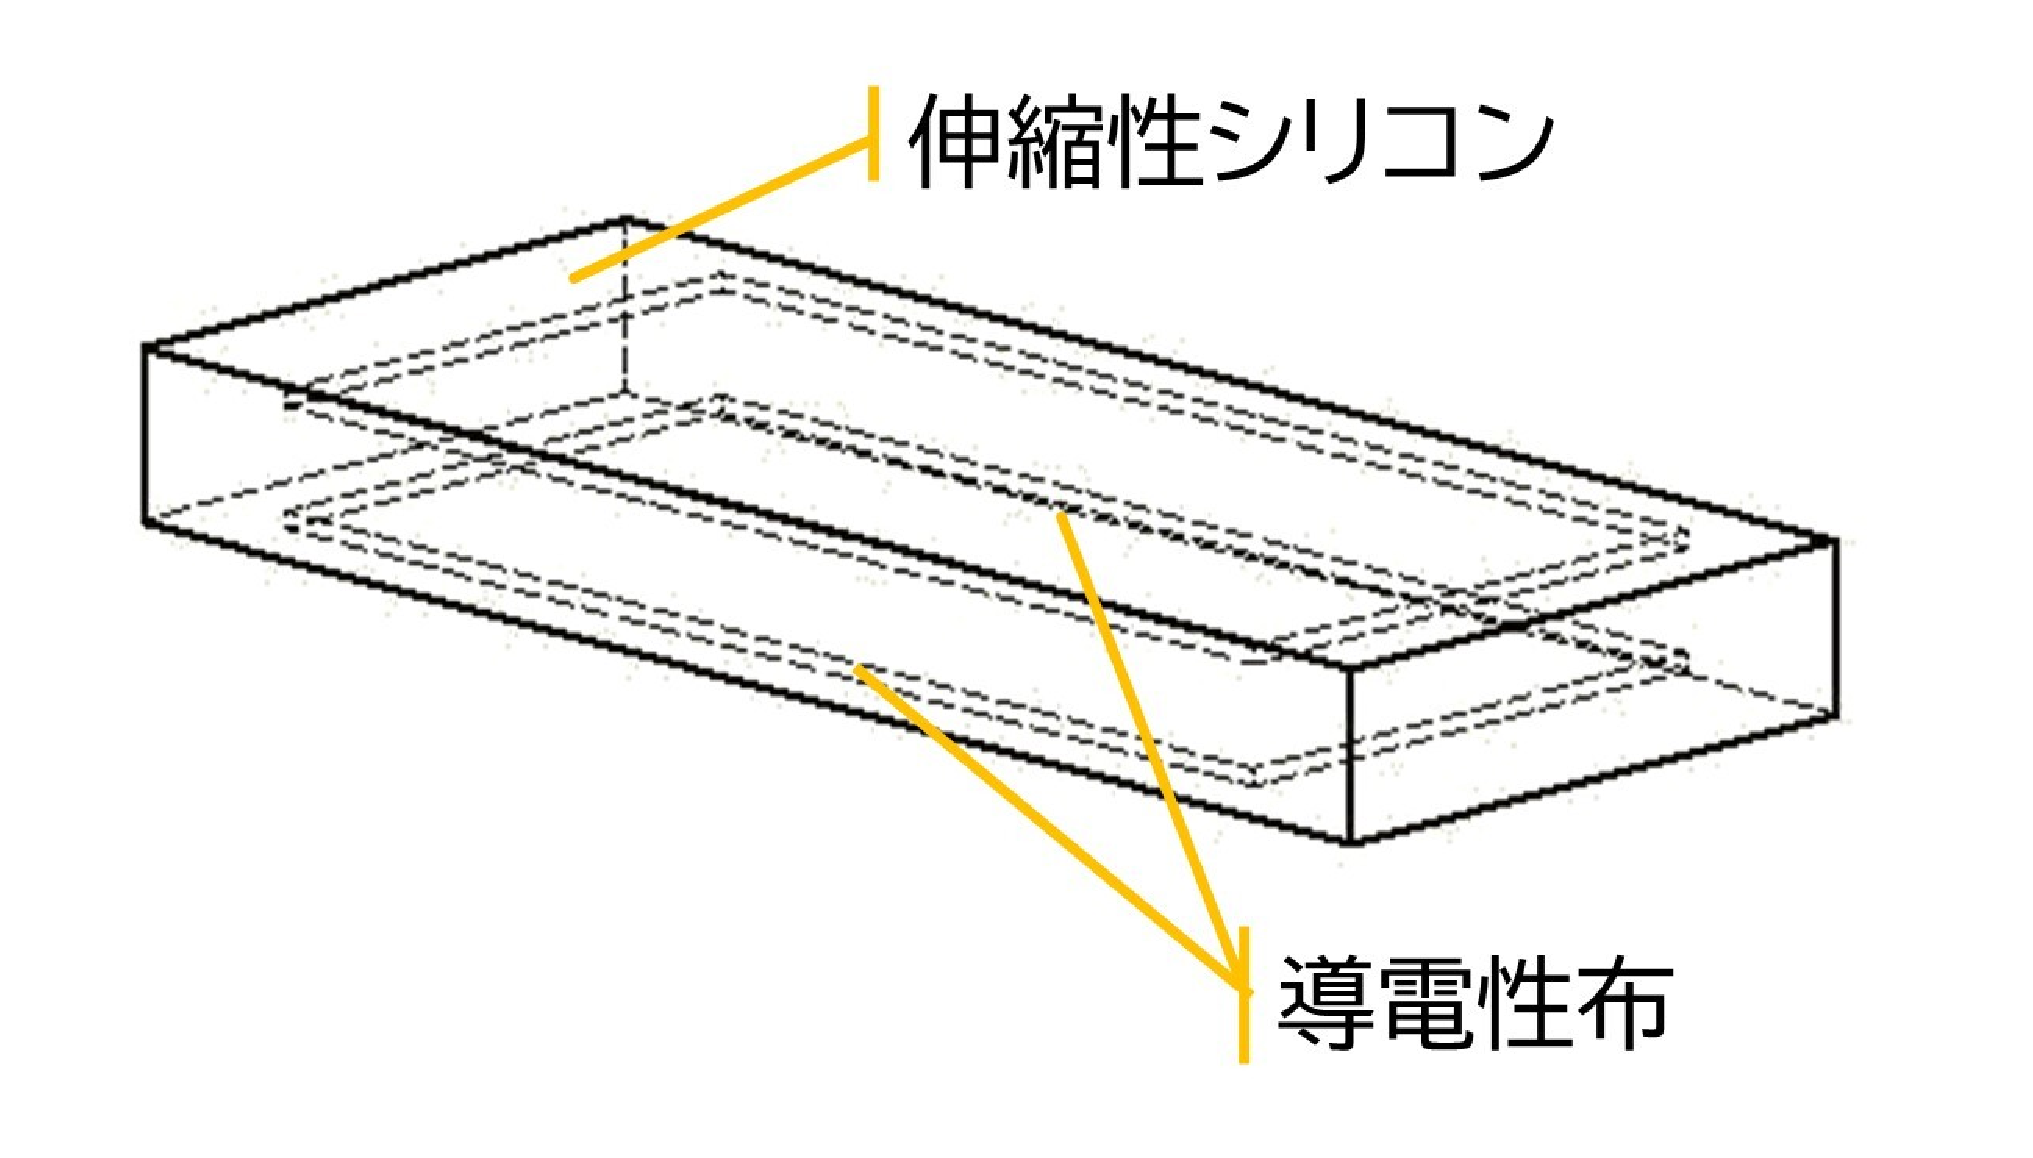
\includegraphics[width=0.5\columnwidth,clip]{Photo/2.実験方法/スライド1.eps}
        \caption{伸縮センサ全体図}
    \end{center}
\end{figure}
\begin{figure}[h]
    \begin{center}       
        \label{伸縮センサ断面図}
        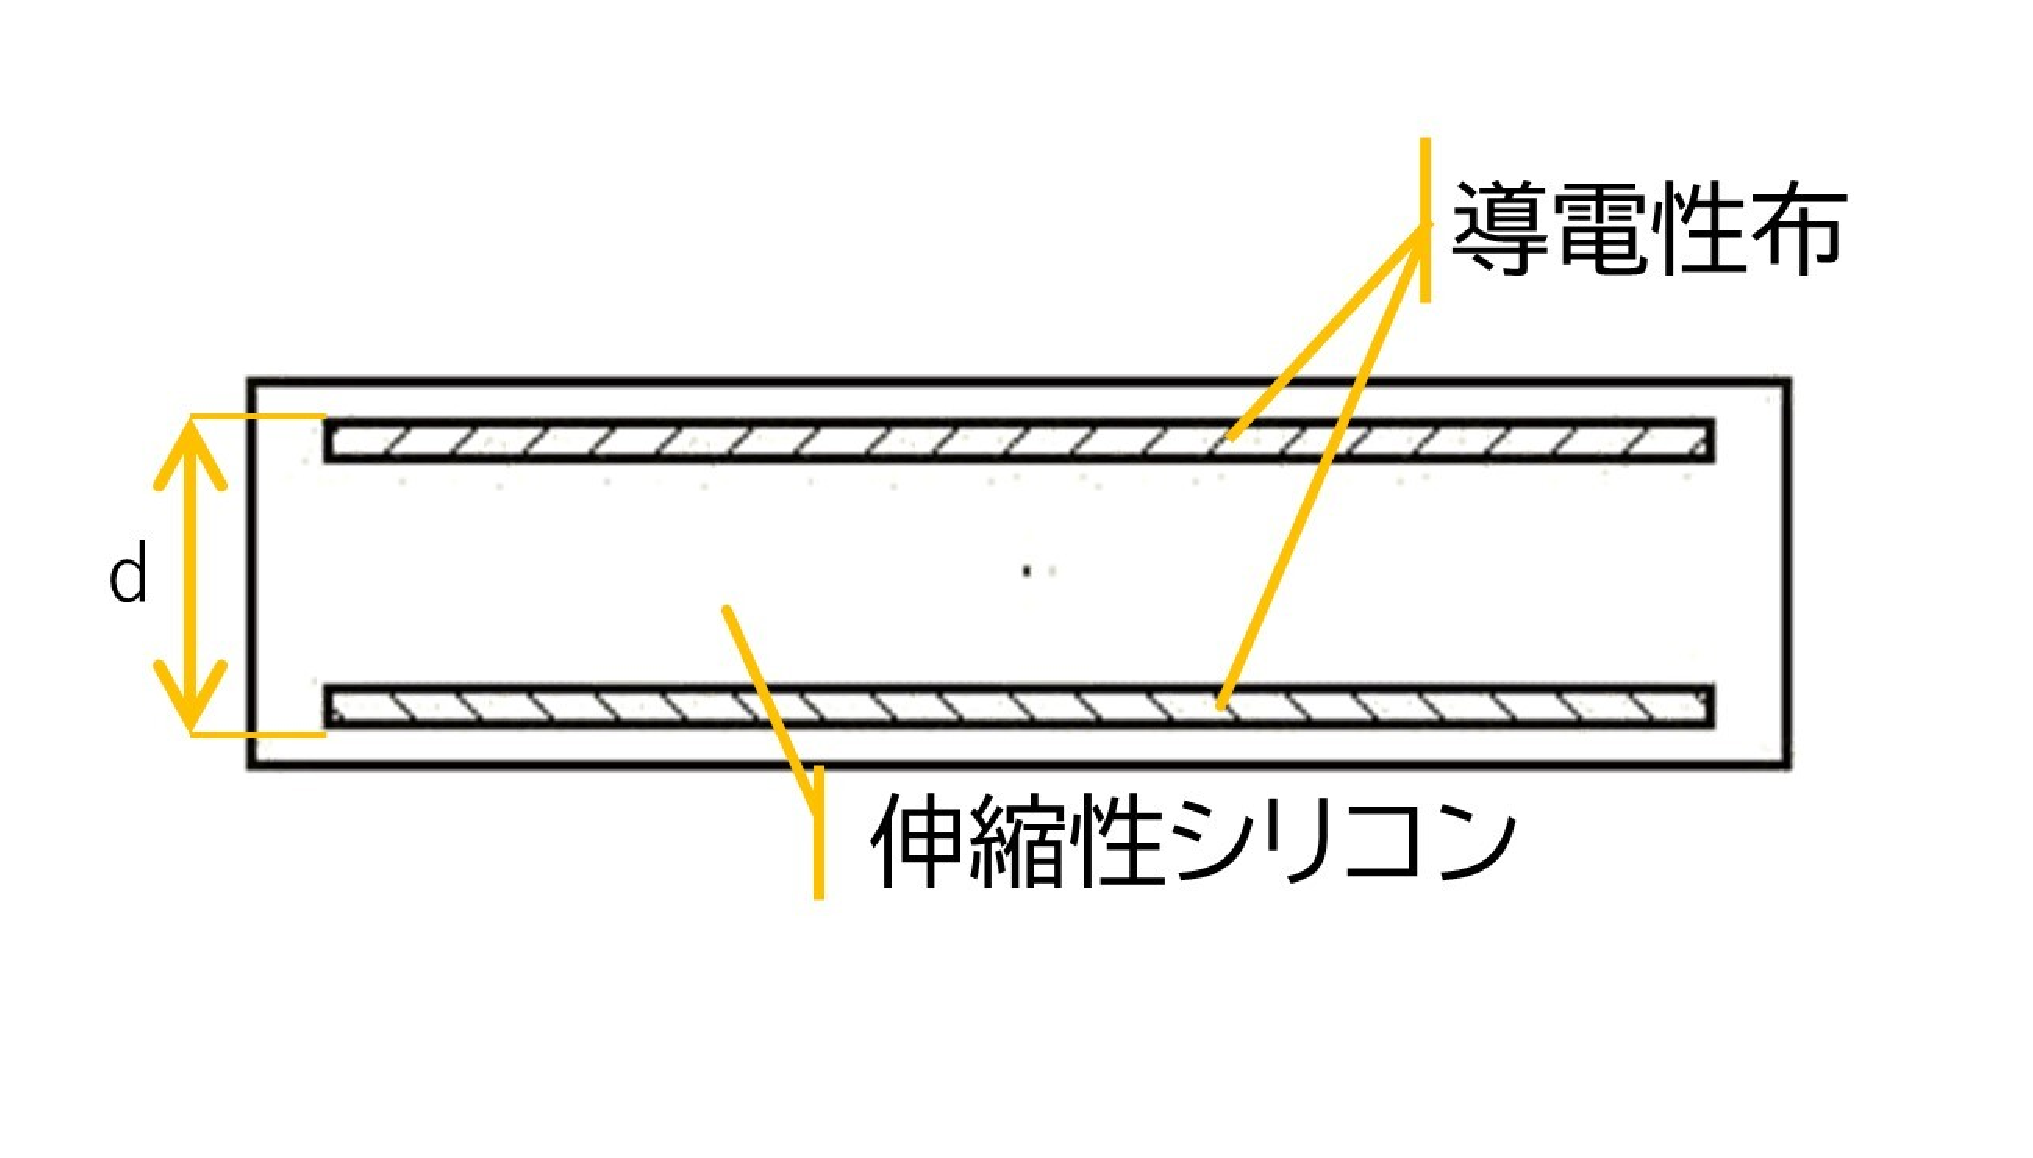
\includegraphics[width=0.5\columnwidth,clip]{Photo/2.実験方法/スライド2.eps}
        \caption{伸縮センサ断面図}
    \end{center}
\end{figure}

\newpage

ここで伸縮センサ中の導電性布の表面積$S$,誘電体の厚さを$d$,真空の誘電率を$\epsilon{}_0$,シリコンの比誘電率を$\epsilon{}_s$とすると,
\begin{eqnarray}
    C=\epsilon{}_0\epsilon{}_s\frac{S}{d}
\end{eqnarray}
といった式となる.ここで体積が一定の変化であると仮定すると,

ここで静電容量の変化を$\Delta{}C$,厚みの変化を$\Delta{}d$とそれぞれすると、

一方で,伸縮センサは引張方向のみに応力がかかる単軸応力状態であると見れるため,引張方向のひずみ$\gamma$,引張方向の垂直応力$\sigma$,ヤング率$E$とそれぞれすると,
\begin{eqnarray}
    \sigma=E\gamma
    \label{フックの法則}
\end{eqnarray}
といった式がフックの法則により示される.また,引張方向に対して直交方向である垂直ひずみ$\gamma{}_s$,ポアソン比$\mu$とすると,
\begin{eqnarray}
    \mu = \frac{\gamma{}_s}{\gamma}
    \label{ポアソン比}
\end{eqnarray}
といった式となる.

\subsection{伸縮センサ計測回路}
%TODO:伸縮センサ計測回路に関しての記述を行う
%TODO:RC回路の電圧を掛けたときの時定数の様子をオシロスコープで撮影した画像が欲しい
先述の通り,伸縮センサは静電容量の変化で伸縮状況を示す.故に今回は静電容量の変化を計測することができる回路の製作を行った.
静電容量の計測を行う方法として、LRCメータやインピーダンスアナライザを用いる方法が挙げられる。
これらの計測機器を用いると静電容量の変化を高精度に計測することができる。しかし、1ch当たりの
計測機器の単価が非常に高く、また既存のフィードバック系に組み込みにくいといった状況があった。そこで、
今回はより安価で手軽な方法である、RC回路を用いた方法をとった。

下記のFig.\ref{RC回路}に示したRC回路を用い、Vinに入力を与えるとVoutで信号が立ち上がるまでに
時間の遅れが発生する。これは、抵抗値$R$、静電容量$C$とすると、時定数$\delta t$は、
\begin{eqnarray}
    \delta t = RC
\end{eqnarray}
といった式であらわされる。

\begin{figure}[h]
 \begin{center}
    %TODO:Voutの向きを出力にする
  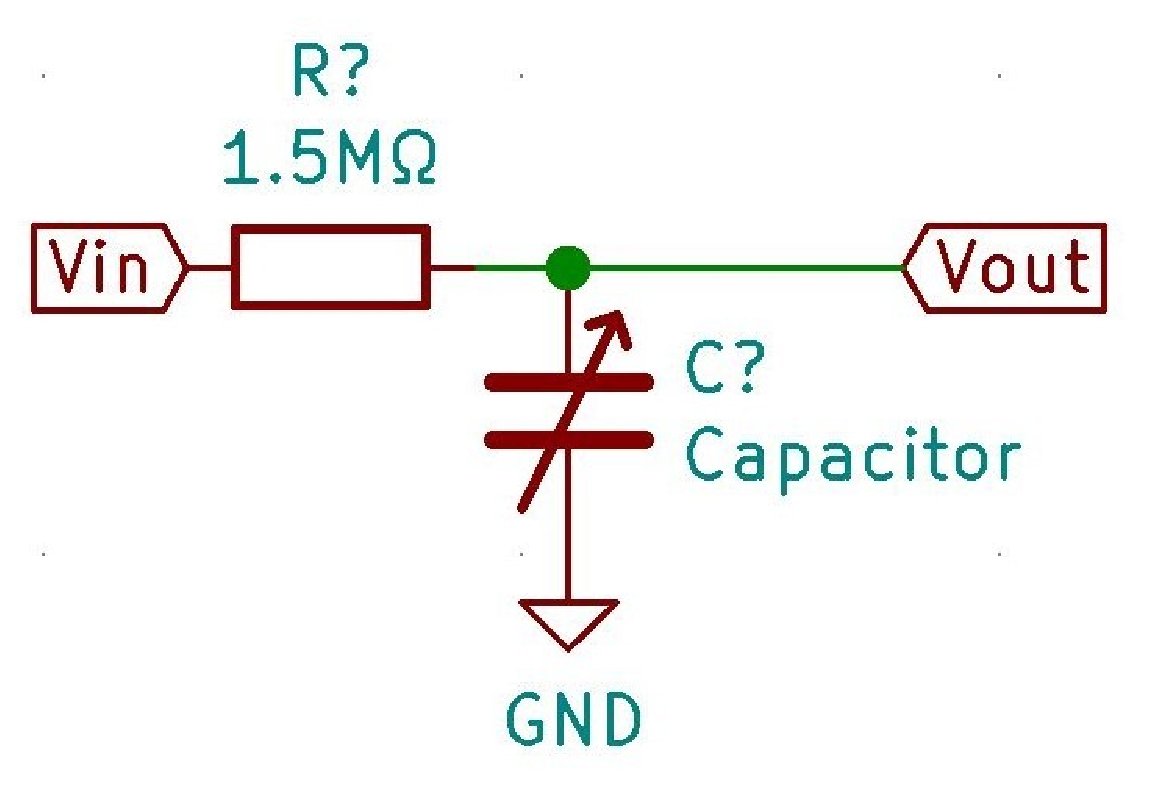
\includegraphics[width=0.5\columnwidth,clip]{Photo/2.実験方法/RC.eps}
  \caption{RC回路}
  \label{RC}
 \end{center}
\end{figure}

\begin{figure}[h]
    \begin{center}
     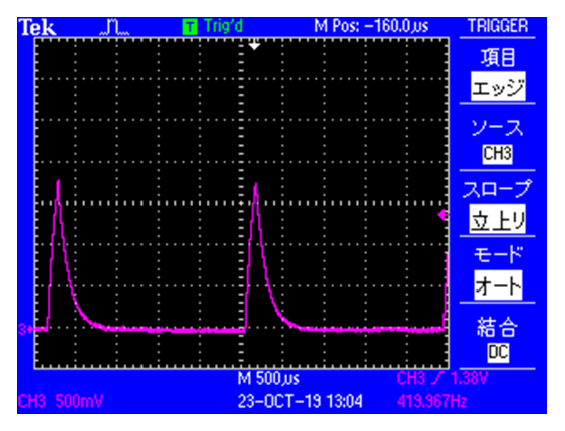
\includegraphics[width=0.5\columnwidth,clip]{Photo/2.実験方法/オシロスコープ.eps}
     \caption{出力状態図}
     \label{オシロスコープ}
    \end{center}
\end{figure}

これらの計測に関して,1つのマイコンを用いて複数の伸縮センサの計測を行うと計測周期が低下し,
計測精度の低下が懸念された.これを踏まえ,1つのマイコンで計測を行う伸縮センサの数を2個とした.
一方で今回,足首を中心とした筋の伸縮の計測を行うため6チャンネル分の計測を行う必要がある.
故に,マイコン3枚分の計測システムを用意した.同期信号を用いて計測のデータ取得,同期を行った.
\begin{figure}[h]
 \begin{center}
  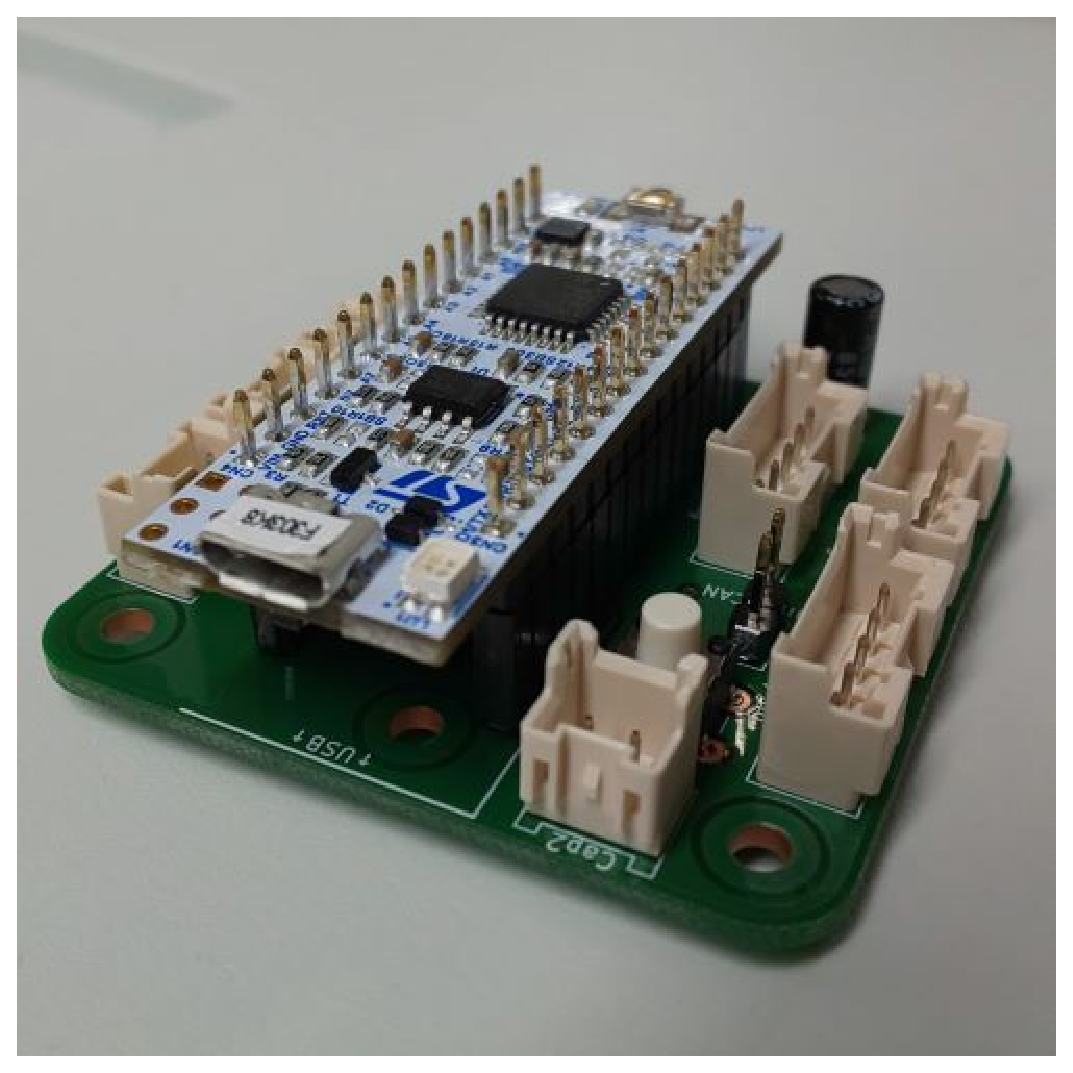
\includegraphics[width=0.5\columnwidth,clip]{Photo/2.実験方法/circuit.eps}
  \caption{計測時に実際に用いた基板}
  \label{circuit}
 \end{center}
\end{figure}